%
% Apunte de Sistemas Operativos
% Copyright (C) 2014 Esteban De La Fuente Rubio (esteban[at]delaf.cl)
%
% Permission is granted to copy, distribute and/or modify this document
% under the terms of the GNU Free Documentation License, Version 1.3
% or any later version published by the Free Software Foundation;
% with no Invariant Sections, no Front-Cover Texts, and no Back-Cover Texts.
% A copy of the license is included in the section entitled "GNU
% Free Documentation License".
%
% Link: http://www.gnu.org/copyleft/fdl.html
%

% PLANIFICACIÓN DE MONOPROCESADORES (CPU)
\chapter{Planificación de monoprocesadores}
\label{planificacion_monoprocesadores}
Durante este capítulo se asumirá que la máquina dispone de una única CPU, o sea,
se discutirá la planificación en monoprocesadores. Considerando este escenario
se analizarán diferentes métodos mediante los cuales el sistema operativo puede
decidir que proceso ocupará el recurso CPU y será ejecutado.

El \textbf{\textit{scheduling}}, o planificación de procesos, corresponde a la
asignación conveniente del recurso CPU a los procesos. Se debe elegir que
proceso tomará la CPU y por cuanto tiempo. La recuperación de la CPU por parte
del sistema operativo se hace mediante una interrupción del cronómetro
regresivo. El \textbf{\textit{scheduler}} de procesos es la componente en el
núcleo, por lo tanto en el área de sistema, que realiza el \textit{scheduling}.

Cada recurso deberá tener su propio planificador y la idea siempre será
favorecer algún tipo de parámetro, como: tiempo de espera u orden de llegada.
Al estudiar y comprender la planificación de procesos para su ingreso a CPU es
posible realizar una analogía con lo que sucede en el resto de dispositivos de
la máquina que requieren algún tipo de planificación para su acceso (donde lo
que generalmente podría cambiar es el algoritmo de desición).

Las \textbf{colas de \textit{scheduling}} pueden ser, por ejemplo, colas FIFO o
con prioridades, donde los procesos esperan por un recurso. El mejor ejemplo es
la cola de procesos listos para ejecutarse en espera de CPU donde el
\textit{scheduler} deberá elegir un proceso de esta cola para la ejecución.
También hay colas para disco donde si un proceso requiere un dato de este deberá
esperar en la cola hasta que el disco esté disponible para ser usado.

Las \textbf{jerarquías de \textit{scheduling}} corresponden a los diferentes
niveles de planificación que pueden existir dentro del sistema operativo,
lo anterior según el proceso y recurso que se debe planificar.
\begin{enumerate}[i.]

% corto plazo
\item \textbf{Corto plazo}: el distribuidor (\textit{dispatcher} o
\textit{scheduler}) es el planificador de mayor frecuencia, el cual debe tomar
decisiones con un mayor de detalle, ya que decide que proceso se ejecutará a
continuación (entrará a la CPU). Se ejecuta cuando ocurre un suceso que lleva a
la interrupción del proceso actual:

\begin{itemize}
	\item Interrupciones del reloj.
	\item Interrupciones de E/S.
	\item Llamadas al sistema operativo.
	\item Señales.
\end{itemize}

% mediano plazo
\item \textbf{Mediano plazo}: elige quién va a la memoria o a disco (evitando
procesos interactivos en disco). Encargado de manejar el intercambio entre los
procesos suspendidos y no suspendidos. Al salir de la cola de mediano plazo
vuelven a la cola a corto plazo para ahora esperar a entrar a la CPU.

% largo plazo
\item \textbf{Largo plazo}: para procesamientos por lotes (o \textit{jobs}). Una
vez lanzado no podrá ser detenido por el \textit{scheduling} de largo plazo y el
\textit{job} se ejecutará hasta el final. Es el que determina cuales son los
programas que serán admitidos para ejecución en el sistema, independientemente
de lo que suceda después en las otras colas (de mediano o corto plazo). Una vez
aceptado el proceso pasará a la cola de corto plazo o mediano plazo (en caso de
comenzar con menor prioridad o suspendido). En sistemas interactivos se aceptan
todos los trabajos hasta que el sistema ya no puede atender a más procesos (dado
por el nivel de multiprogramación y recursos del sistema).
\end{enumerate}

Las \textbf{ráfagas de CPU} corresponden a una secuencia de instrucciones
ejecutadas por un proceso sin pasar a un modo de espera.

Supongamos que en un instante determinado tenemos un proceso $P_2$ en ejecución
y un proceso $P_1$ en un estado WAIT (debido a un requerimiento de E/S). En
algún momento la operación de E/S concluirá pasando a estado READY, sin embargo
el \textit{scheduler} no le asigna la CPU de forma inmediata por lo cual sigue
en estado READY.

\begin{verbatim}
 procesos
    ^
    |
    |wait_io     ready     run    ready       run   wait_io
P1  |......................_______............______.......
    |
P2  |______________________.......____________
    |
    -------------------------------------------------------------> tiempo
\end{verbatim}

Le interrupción (int) del término del proceso de E/S solicitado por el proceso
$P_1$ le llegará al proceso $P_2$, por lo cual la rutina de instrucción que
atiende la interrupción se ejecuta en tiempo de sistema pero dentro del tiempo
real de $P_2$, y es en el tiempo de $P_2$ donde se pasa $P_1$ a estado READY.
Todo esto sin existir cambio de contexto, ya que el tiempo que dura la
interrupción es mucho menor al que toma el hacer un cambio de contexto para que
$P_1$ atienda la interrupción.

Una vez $P_2$ entrega la CPU, por algún motivo, $P_1$ se ejecuta, si se asume un
sistema con procesos donde el sistema operativo puede quitar la CPU, en algún
momento a $P_1$ se le puede obligar a dejar la CPU, para volver a colocar a
$P_2$, luego $P_1$ podrá volver a ejecutarse nuevamente más adelante, esto
seguirá sucediendo hasta que el proceso termine o bien exista alguna espera por
E/S, a menos que alguna de estas dos últimas situaciones ocurra se dirá que la
ráfaga de CPU de $P_1$ serán los estados RUNNING consecutivos sin que exista
WAIT entremedio.

Recordar que una ráfaga de CPU no es una secuencia ininterrumpida de
instrucciones, sino que es una secuencia de instrucciones sin pasar a estados de
espera.

La mayoría de las ráfagas de CPU son cortas en tiempo, si hacemos un histograma
se podría observar algo similar a lo mostrado en la figura
\ref{fig:rafagas_cpu}. Donde se observa una curva, donde los procesos con
menores tiempos de ráfagas son procesos intensivos en E/S, y aquellos con altos
tiempos de ráfagas son intensivos en CPU.

\begin{figure}[htbp]
  % http://www.texample.net/tikz/examples/pgfplots/
	\centering
	\selectlanguage{english}
	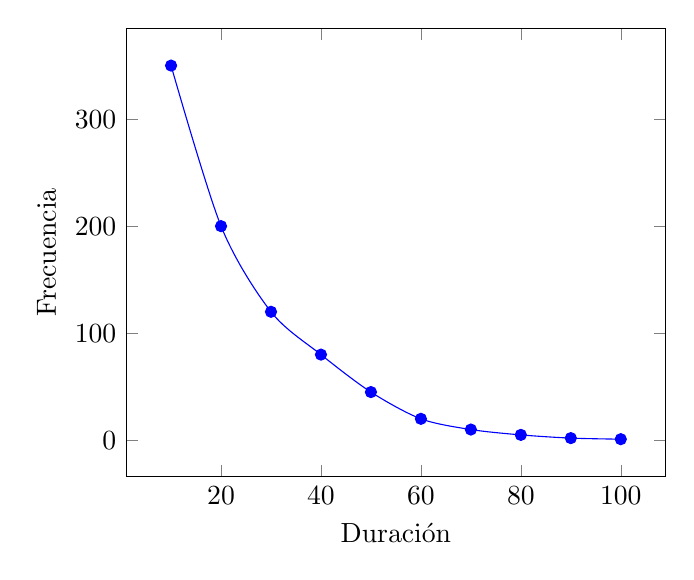
\begin{tikzpicture}
		\begin{axis}[xlabel=Duración, ylabel=Frecuencia]
			\addplot[smooth,mark=*,blue] plot coordinates {
				(10,350)
				(20,200)
				(30,120)
				(40,80)
				(50,45)
				(60,20)
				(70,10)
				(80,5)
				(90,2)
				(100,1)
    	};
		\end{axis}
	\end{tikzpicture}
	\selectlanguage{spanish}
	\caption{Ejemplo ráfagas de CPU}
	\label{fig:rafagas_cpu}
\end{figure}

El objetivo es disminuir la cantidad de cambios de contextos que ocurren en el
sistema y con esto minimizar el sobre costo de los mismos, para esto se debe
fijar una tajada de tiempo adecuada. Según la figura \ref{fig:rafagas_cpu}
sabemos que la mayoría de las tajadas son de duración corta, entonces se les
podría dar a los procesos una tajada de 40 [ms]. De esta forma un proceso tiene
mayor probabilidad de terminar su ráfaga de CPU dentro de la tajada de tiempo,
ya que se asume que la mayoría de los procesos tienen ráfagas menores a 40 [ms].
La estrategia es darle un tiempo lo suficientemente grande para que las ráfagas
se ejecuten de forma contínua, lo ideal es que esto cubra el 80\% de los casos.
Esto corresponde a lo usado en un tipo de \textit{scheduling} el cual es
\textbf{Round-Robin}.

El \textbf{tiempo de despacho} de un proceso corresponderá al tiempo desde que
una ráfaga de CPU se encuentra disponible para su ejecución, o sea el proceso
está en estado READY, hasta que la ráfaga fue atendida por completo. El ideal es
minimizar en los algoritmos la media de los tiempos de cada uno de los procesos
que se están atendiendo. Se definirá el tiempo de despacho total (la media de
todos los procesos) como:

$T_{despacho} = \frac{T_{P1}+T_{P2}+...+T_{Pn}}{n}$

\section{Algoritmos de planificación}

Se deberán fijar criterios para realizar la planificación y de esta forma poder
evaluar cada una de las estrategias posibles a utilizar. Estos criterios pueden
ser:

\begin{itemize}
	\item Tiempo de respuesta.
	\item Tiempo de retorno.
	\item Productividad.
	\item Utilización del procesador.
	\item Equidad.
	\item Prioridades.
\end{itemize}

Los algoritmos de planificación están directamente relacionados con el tipo de
procesos que se estará ejecutando, considerando los tipos \textit{preemptive} y
\textit{non-preemptive}. En aquellas estrategias donde por algún motivo el
sistema operativo puede quitar la CPU al proceso diremos que dicho algoritmo es
del tipo apropiativo y si no la puede quitar será del tipo no apropiativo.

A continuación se describirán algunas de las estrategias de planificación que
puede ser utilizadas en el caso del planificador a corto plazo.

\subsection{FCFS: First Come First Served}

Corresponde al sistema de planificación donde la primera ráfaga de CPU que llega
es la primera que se atiende, o sea, orden FIFO. La ráfaga es ejecutada hasta
que termine su ejecución o bien se bloquee por E/S, por lo cual es un método de
planificación \textit{non-preemptive} (o no apropiativo), mientras el proceso no
pase a un estado de espera, el sistema operativo no podrá utilizar la CPU.

\begin{verbatim}
   ^
   | run                             wait      ready
P1 | ________________________________............................
   | wait      ready                run                   wait
P2 | ................................_____________________.......
   |______________________________________________________________> tiempo
               |---------- tiempo de despacho P2 --------|
\end{verbatim}

Este método presenta el gran problema de que los tiempos de despacho son muy
variables y generalmente largos, lo cual lo hace un sistema de planificación
horrible para sistemas interactivos.

\textbf{Ejemplo}: se tienen 3 ráfagas de procesos de tiempos 24, 3 y 3,
correspondientes a los procesos P1, P2 y P3 respectivamente que llegan en ese
mismo orden a la cola de procesos listos. Se tendrá el siguiente esquema de
planificación:

\begin{verbatim}
P1 ______________
P2 ..............____
P3 ..................____
______________________________ tiempo
   0             24  27  30
\end{verbatim}

$T_{despacho} = \frac{T_{24}+T_{27}+T_{30}}{3} = 27$

Si se planifican de otra forma el tiempo de despacho será diferente, por ejemplo
supongamos el orden P2, P3, P1:

$T_{despacho} = \frac{T_{P1}+T_{P2}+T_{P3}}{Procesos} = \frac{T_{30}+T_{3}+T_{3}}{3} = 13$

\subsection{SJF: Shortest Job First}
En este caso los programadores entregaban un tiempo que se esperaba que durara
el trabajo (\textit{job}), la idea de esto es minimizar la media del tiempo de
despacho de los procesos. Si el tiempo de duración era mayor al esperado
(ejemplo: el doble), se asumía que el proceso estaba caído y se mataba, por lo
que el programador debía colocar un tiempo realista.

La idea es atender primero las ráfagas cortas, no atender el proceso completo de
una vez, sino solo la ráfaga de CPU y con esto minimizar el tiempo de despacho
de dicha ráfaga, minimizando lo que ocurría con FCFS. Para esto se debe estimar
la duración de una ráfaga, la forma de hacer esto es con un promedio ponderado
de la duración de ráfagas anteriores (esto mediante estadísticas del proceso que
lleva el sistema operativo).

Sea:
\begin{itemize}
\item $\tau^{p}_{n+1}$ el predictor para la ráfaga $n+1$ del proceso $p$, el
cual indicará cuanto podría demorar la siguiente ráfaga de CPU del proceso $p$.
\item $\tau^p_n$ la duración de la ráfaga $n$.
\item $\alpha$ ponderados para las duraciones de las ráfagas anteriores.
\end{itemize}

Se puede calcular la duración estimada de la siguiente ráfaga de CPU de un
proceso utilizando la siguiente fórmula, donde $\alpha$ típicamente es un valor
como $0.5$.

$\tau^p_{n+1} = \alpha \tau^p_n + (1-\alpha) \alpha \tau^p_{n-1} + (1-\alpha)^2 \alpha \tau^p_{n-2} + ... + (1-\alpha)^i \alpha \tau^p_{n-i} $

El problema con la fórmula anterior, es que calcular todas las ráfagas
anteriores de todos los procesos es algo muy lento, sin embargo esta fórmula se
puede simplificar ya que es igual a:

$\tau^p_{n+1} = \alpha \tau^p_n + (1-\alpha) \tau^p_n $

En el fondo se va utilizando el cálculo realizado para la ráfaga anterior.
Caso $n=0$ es una condición de borde que es un valor fijo no muy relevante, ya
que al ir teniendo ráfagas se irá calculando el valor real para el proceso.

Este método puede ser \textit{preemptive} o no. Sin embargo si es
\textit{preemptive} se le asigna una cota al proceso a través del \textit{timer}
para introducir un cambio de contexto, donde lo lógico sería utilizar como
tiempo máximo la siguiente ráfaga más corta o bien el predictor calculado, donde
si el proceso excede dicho valor se le quita la CPU. En este caso se ``cubren''
posibles errores que hayan ocurrido al realizar la predicción de la duración de
la siguiente ráfaga del proceso.

Funciona mejor en sistemas interactivos, sin embargo recordar que la motivación
de este método es reducir el tiempo de despacho.

El problema de esto es la hambruna para las ráfagas largas. Esto sucede si
llegan constantemente ráfagas cortas a la cola de listos y nunca se pueden
atender ráfagas más largas.

\subsection{Primero el de menor tiempo restante}
Este caso es muy similar a SJF, sin embargo aquí se evalúa el tiempo que le
queda a cada proceso para terminar su ráfaga y siempre se ejecutará la ráfaga
más corta. Esto significa que si tenemos un proceso en ejecución y entra un
proceso a la cola de listos cuya ráfaga siguiente es más corta que la que está
actualmente ejecutándose habrá un cambio. Por lo anterior este método es
apropiativo.

\subsection{Primero el de mayor tasa de respuesta}
En este tipo de estrategia se define una tasa de respuesta (o \textit{response
ratio}) como $RR = (w + s) / s$, donde $w$ es el tiempo que el proceso lleva
esperando por el procesador y $s$ es el tiempo total de servicio esperado para
la ráfaga que se esta atendiendo.

Este método entregará la ``edad'' del proceso, donde entrarán al procesador
aquellos que lleven más tiempo esperando por el uso de CPU.

Si en algún momento el proceso que se está ejecutando deja de ser el de mayor
``edad'', porque otro lleva más tiempo esperando, la CPU le será quitada y
asignada al otro proceso. Por esta razón esta política es apropiativa.

\subsection{Prioridades}
En este método se ejecuta de la cola de listos el proceso con mejor prioridad.
Se manejarán diferentes colas listas, cada una representará un nivel de
prioridad diferente y los procesos de prioridades inferiores no serán atendidos
hasta que se hayan atendido los de la prioridad superior, ver figura
\ref{fig:planificacion_prioridades}.

\begin{figure}[htbp]
\centering
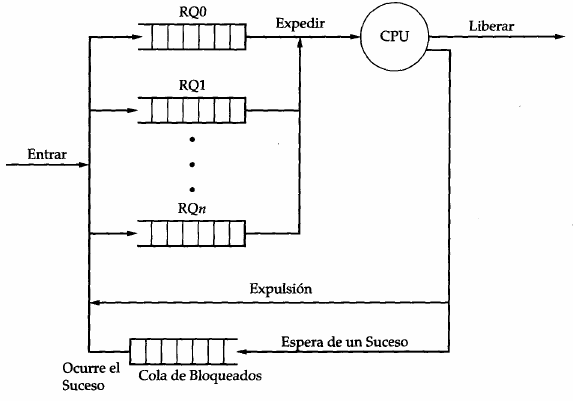
\includegraphics[scale=.9]{img/C06_cpu/prioridades.png}
\caption{Planificación considerando colas de prioridades ($RQ0$ a $RQn$)}
\label{fig:planificacion_prioridades}
\end{figure}

Los casos anteriores (excepto FCFS) son casos particulares de prioridades, por
ejemplo en SJF la prioridad del proceso es su predictor $\tau^p_{n+1}$.

La idea de utilizar prioridades pretende que el sistema pueda ser sensible
frente a las situaciones que en el están ocurriendo, donde un sistema podrá ir
adecuandose a la forma en la que se van ejecutando los procesos.

En general el problema de esta solución es la hambruna, donde procesos con peor
prioridad pueden no ser atendidos nunca.

La solución para la hambruna consiste en utilizar una variante llamada
\textbf{\textit{aging}} (añejamiento), donde cada cierto tiempo se mejora
temporalmente la prioridad de todos los procesos que están en la cola listos.
Ejemplo, cada 10 [ms] hay una interrupción y se mejora la prioridad a todos los
procesos, con esto se espera que después de un tiempo $X$ el proceso alcanzará
la prioridad necesaria para entrar a la CPU. Una vez se concede el acceso a la
CPU y el proceso sale, este retoma su prioridad original.

Otra técnica para evitar la situación de hambruna es el uso de prioridades con
retroalimentación, donde una vez que el proceso ha sido atendido por la CPU al
salir de esta pasará a una cola de menor prioridad. Esto con el objetivo de
permitir que otros procesos puedan entrar a la CPU, ver figura
\ref{fig:planificacion_realimentacion}.

\begin{figure}[htbp]
\centering
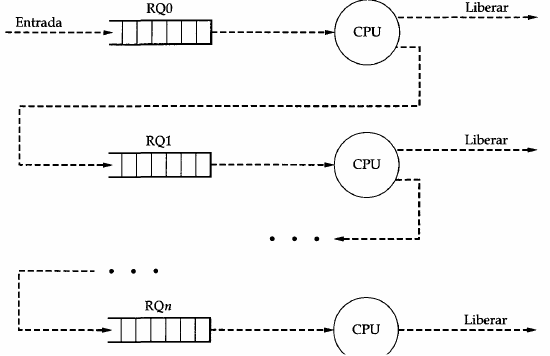
\includegraphics[scale=.9]{img/C06_cpu/realimentacion.png}
\caption{Planificación considerando colas de prioridades con realimentación}
\label{fig:planificacion_realimentacion}
\end{figure}

\subsection{Round Robin}
Se busca minimizar el tiempo de respuesta y es la estrategia de planificación
utilizada hoy en día. Se diseñó específicamente para sistemas de tiempo
compartido, los cuales típicamente son interactivos.

El \textbf{tiempo de respuesta} en sistemas interactivos es el tiempo que
transcurre desde que el usuario inicia una interacción hasta observar el primer
resultado. Si un comando entrega una serie de líneas, el tiempo entre línea y
línea será el tiempo de respuesta.

Psicológicamente se mostró que al usuario le interesa ir viendo resultados, o
sea ir viendo que aparecen líneas avanzando en la pantalla. Un comando que se
demora 10 segundos, pero estuvo entregando durante los 10 segundos respuestas es
mejor, psicológicamente, que un comando que duro 5 segundos, pero durante esos 5
segundos no se entregó ninguna respuesta por la pantalla, sino solo hasta el
final.

En este método de planificación los procesos forman una lista circular y el
\textit{scheduler} da tajadas de tiempo, típicamente de 10 a 100 [ms], a cada
uno de los procesos.

\textbf{¿Cuál es el tamaño de la tajada de tiempo?} Si es muy grande se
parece a FCFS, si es muy pequeña habría un costo excesivo en el cambio de
contexto. Regla empírica, el 80\% de las ráfagas de CPU deben durar menos que el
tiempo de la tajada.

En este tipo de \textit{scheduling} la decisión crítica es \textbf{¿qué hacer
con las ráfagas que llegan?}, ya que cuando la ráfaga llega uno podría proponer:

\begin{enumerate}[i.]

\item Se otorga inmediatamente la CPU a dicho proceso con la tajada de tiempo
completa (de bloqueado a listo), esto tiene sentido porque un proceso que estaba
en estado de espera, el mismo cedió la CPU para ingresar al estado de espera. El
problema, según como sea el \textit{scheduling}, procesos que son intensivos en
lectura escritura podrían causar hambruna a los que son intensivos en CPU.

\item Para evitar la hambruna, se puede adoptar que cuando un proceso pase a
estado de espera, al recibir el recurso, no recibe la tajada completa, sino lo
que le quedaba de tajada. El problema con esto, hay muchos cambios de contexto
si los procesos son intensivos en E/S.

\item Otra variante, para minimizar el cambio de contexto, el proceso se deja
para más adelante ubicándolo al final o al inicio. Cada una con sus problemas,
la primera lo desfavorecería, la segunda podría provocar cierta hambruna en
procesos que son intensivos en CPU.

\end{enumerate}

El debate es ¿cómo minimizar el sobre costo de cambios de contexto dando uso
equitativo de la CPU?

\section{Planificación en Linux}
El \textit{scheduling} en sistemas Unix se realiza utilizando el sistema de
prioridades más el uso de \textit{aging} (para evitar hambruna). En caso de
procesos de misma prioridad se utiliza Round Robin.

Para efectos de planificación los procesos son clasificados en 3 grupos:
\begin{itemize}
\item Procesos batch: sin interacción con el usuario, generalmente en segundo
plano (ej: compiladores, base de datos).
\item Procesos interactivos: interacción continua con los usuarios, deben ser
procesos atendidos rápidamente (ej: editor de textos).
\item Procesos de tiempo real: tiempo corto de respuesta (ej: video, audio,
sensores externos).
\end{itemize}

Es difícil determinar si un proceso es batch o interactivo, por lo cual se
utilizan estadísticas basadas en el comportamiento previo de un proceso para
determinar a que tipo corresponde.

Además los procesos pueden ser clasificados como:

\begin{itemize}
\item Procesos convencionales: interactivos y batch.
\item Procesos no convencionales: tiempo real.
\end{itemize}

``Para poder determinar qué proceso se debe ejecutar a continuación, el
planificador de Linux  busca  en  la lista  no  vacía  con  la prioridad
estática más alta y toma el proceso a la cabeza de dicha lista. La política de
planificación determina para cada proceso, dónde se insertará en la lista de
procesos, con qué prioridad estática y cómo se moverá dentro de esta
lista.''\footnote{Citado textualmente desde man}

Los algoritmos de scheduling encontrados dentro del núcleo Linux son:
\begin{itemize}
\item SCHED\_FIFO: cola estándar para procesos en tiempo real, mientras no haya
un proceso de prioridad mayor el proceso tendrá la CPU.
\item SCHED\_RR: tiempo compartido en tiempo real, asignación justa a procesos
con igual prioridad.
\item SCHED\_OTHER: planificador de tiempo compartido universal.
\item SCHED\_BATCH: para procesos convencionales cuando el procesador esta
``inactivo''.
\end{itemize}

\subsection{Planificación de procesos convencionales}
Para asignar la prioridad se monitorean los procesos y según lo que van haciendo
son favorecidos o penalizados en su prioridad (dependiendo de si han obtenido o
no la CPU). Se distinguen 2 tipos:

\begin{itemize}
\item Estática: asignada inicialmente a un proceso, no responde a los cambios
del sistema (heredada del proceso padre).
\item Tiempo real o dinámica: responde a los cambios del sistema, y al
comportamiento del proceso.
\end{itemize}

Ambas prioridades se mueven entre los valores 100 (mejor prioridad) y 139 (peor
prioridad).

\subsubsection{Prioridad estática}
Para procesos convencionales se utiliza una prioridad estática, que va desde 100
a 139. Esta se verá afectada por el comando \textit{nice} o la llamada a sistema
\textit{setpriority}. Esta prioridad ayudará a determinar el ``quantum'' base
del proceso, de tal forma que:
\begin{itemize}
\item $PE < 120 => quantum = (140 - PE) * 20 [ms]$
\item $PE >= 120 => quantum = (140 - PE) * 5 [ms]$
\end{itemize}

\subsubsection{Prioridad dinámica}
La prioridad dinámica es calculada según el comportamiento del proceso en el
sistema, donde, según como sea este, recibirá un \textit{bonus} para mejorar o
empeorar su prioridad. Al igual que con la prioridad estática su valor va entre
100 y 139. El planificador buscará por esta prioridad al momento de elegir un
proceso para que entre a la CPU.

Se define como: $PD = max (100, min (PE - bonus + 5, 139))$, donde  el bonus es
un valor de 0 a 10, relacionado con el tiempo de \textit{sleep} promedio del
proceso.

Ejemplo: $PD = max (100, min (120 - 5 + 5, 139)) = 120$

El \textbf{tiempo de \textit{sleep}} corresponde a un promedio del tiempo que el
proceso ha pasado durmiendo (sin entrar a la CPU). Este tiempo decrece mientras
un proceso esta corriendo y será como máximo 1000[ms], independientemente del
tiempo real que lleve sin entrar a CPU. El bonus se define utilizando el tiempo
de \textit{sleep} como : $bonus = floor ( tiempo / 100 )$.

Utilizando este tiempo de \textit{bonus} se puede determinar si un proceso es
interactivo o batch utilizando la siguiente fórmula $bonus – 5 >= PE / 4 - 28 =>
interactivo$. Por la fórmula anterior tenemos que un proceso con prioridad
estática \textit{default} (o sea 120) al iniciar no será considerado
interactivo, solo aquellos con una prioridad mejor (o sea 119 o menos). ¿Cuándo
un proceso con prioridad \textit{default} será considerado interactivo?

\subsection{nice}
\textit{nice} permite empeorar (o mejorar) la prioridad estática de un proceso,
esto permitirá ajustar el valor entre 100 y 139, sin embargo para mejorar la
prioridad se requieren privilegios de administrador (usuario \texttt{root}). Lo
anterior ya que la idea original de \textit{nice} era que un usuario fuese
amable (\textit{nice}) con otros al bajar la prioridad de sus procesos.

Los parámetros de la instrucción van de -20 a 19, donde, como ya se mencionó
valores negativos solo puede asignarlos \textit{root}. La nueva prioridad se
calculará como $PE nueva = PE default (120) + nice$.

\subsubsection{Ejemplo}
A continuación se adjunta un ejemplo en C que afecta la prioridad estática de
un proceso. Se sugieren distintas formas de ejecución con diferentes resultados.

\begin{lstlisting}
#include <sys/time.h>
#include <sys/resource.h>
#include <stdlib.h>
#include <stdio.h>
int main (int n, char* args[]) {
    // crear variables para guardar las prioridades
    int prioridadActual, prioridadNueva;
    // determinar prioridad nueva
    if(n==2) prioridadNueva = atoi(args[1]);
    else prioridadNueva = 0;
    // mostrar prioridad con que se llamo al proceso
    prioridadActual = getpriority(PRIO_PROCESS, 0) + 120;
    printf("Prioridad original: %d\n", prioridadActual);
    // cambiar prioridad y mostrarla
    setpriority(PRIO_PROCESS, 0, prioridadNueva);
    prioridadActual = getpriority(PRIO_PROCESS, 0) + 120;
    printf("Prioridad cambiada: %d\n", prioridadActual);
    // salir del programa
    return EXIT_SUCCESS;
}
\end{lstlisting}

\begin{enumerate}[i.]
\item Compilar: \texttt{\$ gcc -Wall prioridad.c -o prioridad}
\item Ejecutar normal: \texttt{\$ ./prioridad}
\item Ejecutar con nice: \texttt{\$ nice -n 10 ./prioridad}
\item Pasar prioridad como parámetro: \texttt{\$ ./prioridad 5}
\item Ejecutar con nice y pasar prioridad como parámetro: \texttt{\$ nice -n 7
./prioridad 3}
\end{enumerate}

¿Qué pasa en el último caso con el valor 3?

\section{Ejercicios y preguntas}
\begin{enumerate}
\item ¿Cuál es la función de las políticas de \textit{scheduling}?
\item ¿Qué tipo jerarquías de planificación existen? Explíquelas.
\item ¿Qué jerarquía es la encargada de elegir el proceso que entrará a la CPU?.
\item ¿Qué condición se debe dar en la ejecución de un proceso para que se
considere que dicha ejecución corresponde a solo una ráfaga de CPU?.
\item ¿Qué es el tiempo de despacho de un proceso?
\item Nombre tres criterios que se pueden utilizar para determinar la estrategia
de planificación a utilizar.
\item ¿Cuál es la diferencia entre políticas de planificación apropiativas y no
apropiativas?
\item ¿FCFS es apropiativo o no apropiativo?
\item ¿Cuál es el gran problema de FCFS?
\item En FCFS, los procesos ¿son todos atendidos?
\item El orden en que llegan las ráfagas en FCFS ¿afectará el tiempo de
despacho? Explique con un ejemplo.
\item ``Primero el trabajo más corto'', ``primero el de menor tiempo restante''
y ``primero el de mayor tasa de respuesta'' ¿son casos particulares de qué
estrategia de planificación?.
\item En SJF, ¿qué es y qué representa el predictor de la ráfaga?.
\item La tasa de respuesta (o \textit{response ratio}) de un proceso, ¿con qué
esta relacionada?.
\item ¿Por qué la estrategia de prioridades presenta hambruna?, explique.
\item ¿Qué técnica se puede utilizar en una planificación con prioridades para
evitar la hambruna?.
\item ¿Por qué es crítico definir de forma correcta la tajada de tiempo en Round
Robin?.
\item ¿Qué tipo de planificación se utiliza en el sistema operativo Linux?.
\item ¿Para que es utilizada la prioridad estática de un proceso en Linux?.
\item ¿Para que es utilizada la prioridad dinámica de un proceso en Linux?.
\item En la prioridad dinámica se utiliza un \textit{bonus} para mejorar o
empeorar esta, ¿de qué depende este \textit{bonus}?.
\item ¿Cuál es la prioridad estática por defecto?.
\item ¿Qué usuarios pueden mejorar la prioridad estática de sus procesos?.
\end{enumerate}

\section{Referencias}
\begin{itemize}
\item Sistemas Operativos, Segunda Edición, Andrew Tanenbaum, Capítulo 2.4.
\item Sistemas Operativos, Quinta Edición, Abraham Silberschatz y Peter Baer
Galvin, Capítulo 5.
\item Sistemas Operativos, Segunda Edición, William Stallings, Capítulo 8.
\end{itemize}
